\documentclass[conference]{IEEEtran}
\IEEEoverridecommandlockouts
% The preceding line is only needed to identify funding in the first footnote. If that is unneeded, please comment it out.
\usepackage{cite}
\usepackage{amsmath,amssymb,amsfonts}
\usepackage{algorithmic}
\usepackage{graphicx}
\usepackage{textcomp}
\usepackage{xcolor}
\usepackage{url}
\def\BibTeX{{\rm B\kern-.05em{\sc i\kern-.025em b}\kern-.08em
    T\kern-.1667em\lower.7ex\hbox{E}\kern-.125emX}}
\begin{document}

\title{Emotional Recognition on Twitter\\
{\footnotesize CPSC 571 Group 14}
}

\author{\IEEEauthorblockN{1\textsuperscript{st} Matthew Forman}
\IEEEauthorblockA{\textit{dept. Computer Science} \\
\textit{University of Calgary}\\
Calgary, Canada \\
matthew.forman@ucalgary.ca}
\and
\IEEEauthorblockN{2\textsuperscript{nd} Firoz Lakhani}
\IEEEauthorblockA{\textit{dept. Computer Science} \\
\textit{University of Calgary}\\
Calgary, Canada \\
firoz.lakhani1@ucalgary.ca}
\and
\IEEEauthorblockN{3\textsuperscript{rd} Rohan Chaudhary}
\IEEEauthorblockA{\textit{dept. Computer Science} \\
\textit{University of Calgary}\\
Calgary, Canada \\
rohan.chaudhary@ucalgary.ca}
}

\maketitle

\begin{abstract}
This report is going to cover the implemenation of an algoirthm that is used to determine the sentiment and emotion behind a given tweet.
We will discuss the pros and cons of existing methods and how a hybrid of these existing methods could create a more usable result.
Social media is a space which is utilized to express many sentiments and emotions. 
In many real world applications, it is important to identify these emotions efficiently and as accurately as possible. 
The ability to identify and predict emotional tone and public perception of various issues can be useful in many scenarios. 
For example, being able to differentiate between sarcasm and a person being serious on twitter can be difficult at times. 
With accurate emotional recognition algorithms, one may be able to understand when something is sarcasm vs when it is not and avoid some of the stress and anger a post may instill otherwise. 
As well, there is incentive from large corporations and governments to understand how the public is perceiving a new product or service. 
With this new knowledge, products and services could theoretically be changed to help positively effect the most amount of people. 

\end{abstract}

\section{Introduction}
Twitter (now X) is one of the most popular forms of social media on the planet.
With the immense amount of traffic it receives it can be thought of as a great tool to monitor how individuals feel about certain topics.
With the help of AI and Machine Learning Models, it is possible to decipher between the sentiment behind a given tweet.
When this done on a mass scale it can be used to figure out how the public feels on a given topic.
However, one problem with this being done on a mass scale is the time it takes to compute and train the models.
The model used in this report is the BERTweet model.
While this model is known to be very accurate the computing power necessary to run this model is very high.
As a result of this model on a database of tweets can take quite some time unless one has an incredibly powerful computer.
Therefore, this leaves an opportunity to combine the technology behind this modern model with some quicker existing machine learning algorithms.
This other machine learning algorithm is the Support Vector Machine (SVM) algorithm.
This method combined with the embeddings established by the BERTweet model could result in a much quicker analysis of the tweets.
On top of this, having visualizations of the analysis of the tweets is essential for understanding the data properly.
Without proper visualizations interpreting the data can be more difficult than necessary. 
Our proposed solution for this will include testing BERTweet, a hybrid of BERTweet embeddings and SVM as well as Normal SVM. 
On top of this we will display the results of the calculations on a webpage with several visualizations for the data. 
With this in mind we hope to cover some gaps in the existing implementations through adapting to lower computing power and displaying the results in a more friendly manner. 


\section{Literature Review}
There are many current studies that have also had intentions to create an algorithm to assign sentiment to tweets.  
From these studies, the following has been discovered.
Assigning sentiment should be split up into three categories, positive, neutral, and negative.
This separation of tweets has been used in several sentiment analysis studies.
For example this was the way tweets were separated in a study by Samah Jailani, Hamzah, Amunuddin, Abidin, and Riza in which there algorithm "establishes whether a particular tweet is supportive, critical, or neutral\cite{b2}."
Emotion can also be assigned to tweets, these being split up into sections of anger, sadness, joy, fear, and disgust. 
In a study by Benrouba, and Boudour, IBM's natural language understanding API tool was used to analyze words associated with positive, negative and neutral emotions\cite{b1}.
This tool assigns values between 0 and 1 for emotions mentioned above per word. 
From here, tweets were analyzed to calculate distance to these baseline words in an unsupervised fashion in order to identify the sentiment behind it. 
As well, there were implementations of this algorithm that focussed on deciphering the sentiment or emotion of a tweet on an individual scale, or on a more mass tweet scale.
The analysis in bulk was done mainly to understand how the public was perceiving a certain topic of interest online. 
Whereas the individual assessment was more focussed on understanding how one person felt in general based on the sentiment behind their tweets. 
Through analyzing existing papers some pros and cons with existing methodologies were established. \newline
\newline
Pros: 
\begin{itemize}
    \item Proven accuracy of SVM algorithm.
    \item Proven accuracy of BERTweet Self-supervised Algorithm.
\end{itemize}
Cons:
\begin{itemize}
    \item Much fewer studies in which unsupervised algorithms were tested in this context.
    \item There is a lot of overlap between neutral, and positive and negative key words making it harder to determine sentiment.
    \item Very little in the way of good visualizations for the output of the algorithms.
\end{itemize}

As mentioned above, Taking an SVM approach was one of the most accurate in terms of supervised algorithms.
It outperformed other algorithms of Sentiment Analysis across multiple examined studies. 
An SVM works by identifying "a hyperplane that distinctly segregates the data points of different classes \cite{b6}." 
What this means is the data is expanded onto a multidimensional plane that is split up by the hyperplane. 
The hyperplane will have margins that expand to the size of the closest data point to it that falls immediately after the hyperplane center. 
This makes decision-making faster and more efficient. 
\begin{figure}[t]
    \centerline{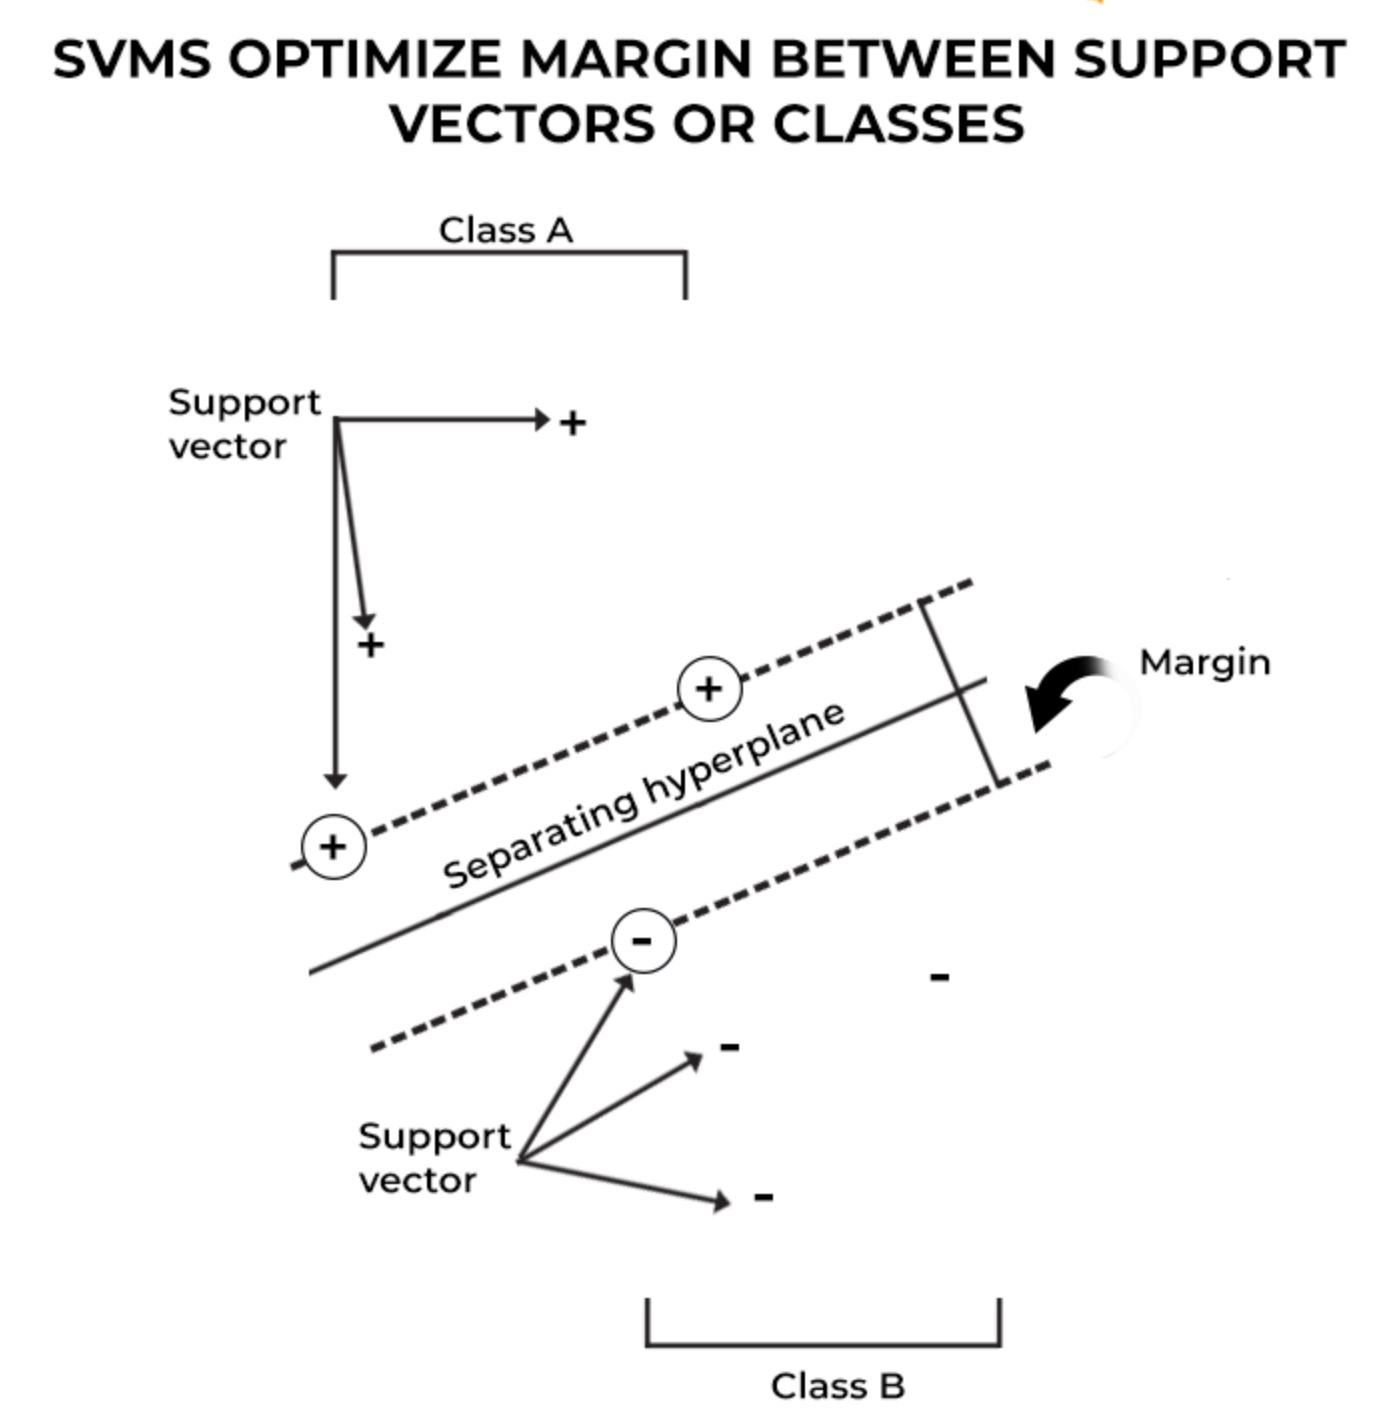
\includegraphics[width=0.5\textwidth]{SVMVisualization.png}}
    \caption{Visualization of hyperplane from SVM \cite{b6}.}
\end{figure}
With modfications this strategy has been used not only to cover binary data, but through using a method called a "kernel trick\cite{b6}" it is used on multidimensional data as well. 
Using this technique achieved very impressive accuracy levels on sentiment analysis of tweets according to other studies.
For example, in the study by Kavitha, Prasad Reddy, and Venkata Rao, it was observed that "SA [Sentiment Analysis] using SVM classifiers is varying between 90.1 and 94.8\%\cite{11}."
As well, in the study by Susmitha, Nikhul, Akhil, Kavitha, Reddy, and Shailaja, SVM had an accuracy percentage of 82\%\cite{b5}. 
Despite the success of this algorithm with studies seeing accuracy levels in the 90th percentile there is still a much smaller amount of knowledge on how a new style of algorithm would keep up.
A newer "self-supervised\cite{b7}" algorithm that has burst onto the scene is BERT.\newline 

BERT is an example of a self-supervised model. 
What this means is that it uses the data input to train on like a supervised algorithm however the training of the algorithm is done in an unsupervised fashion.
"The unsupervised problem is transformed into a supervised problem by auto-generating the labels\cite{b9}" for the supervised algorithm.
In a study performed by Ionut-Alexandru and Stelian a hybrid of a "BERT and SVM Ensemble Model\cite{b8}" was used to detect emotions.
From this study they found very accurate results from combining the power of BERT and SVM with accuracies in the 90th percentile.
From their results, the overall accuracy for their ensemble was 91\% \cite{b8}.
However, their results for BERT were 89\% \cite{b8}, which is very comparable to that of their ensemble.
These results can be seen in Figure 2.
This leads to the possibility of with different training and potentially more specific topics on tweets better results for BERTweet.

\begin{figure}[b]
    \centerline{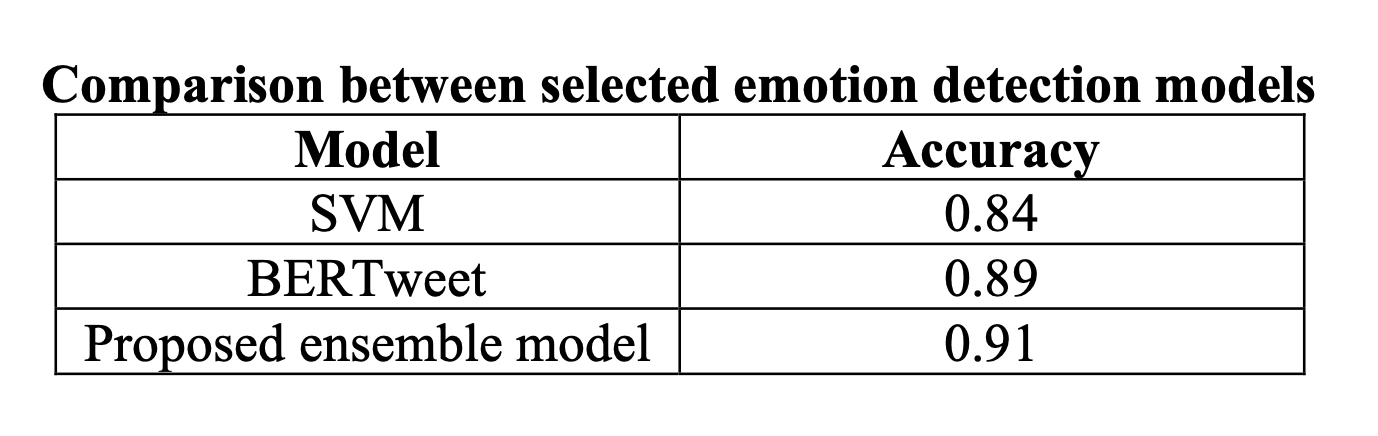
\includegraphics[width=0.5\textwidth]{BERTweetChartFromStudy.png}}
    \caption{Results from Study from Ionut-Alexandru and Stelian\cite{b8}}
\end{figure}

While these results are impressive, proper visualizations of the results were not available other than in the format of these tables.
In a study mentioned above by Samah, Jailani, Hamzah, Aminuddin, Abidin, and Ria, more time was spent on displaying the data to users nicely.
Several different types of charts including pie charts, bar graphs, and histograms were used to clearly visualize the data.
This makes understanding the algorithms decision on what the public feels on a certain topic much easier compared to numbers in a chart.
An example of these charts can be seen in Figure 3. 
As well, in a study by Harshit D. Bhavani, they also created a web application to visualize the data\cite{b3}. 
However, both of these models have never used BERT or any other self-supervised algorithms with these visualizations.
This leaves a gap in the existing studies of nicely presented data using algorithms with superior accuracy, that may be able to be filled. 

\begin{figure*}[t]
    \centering
    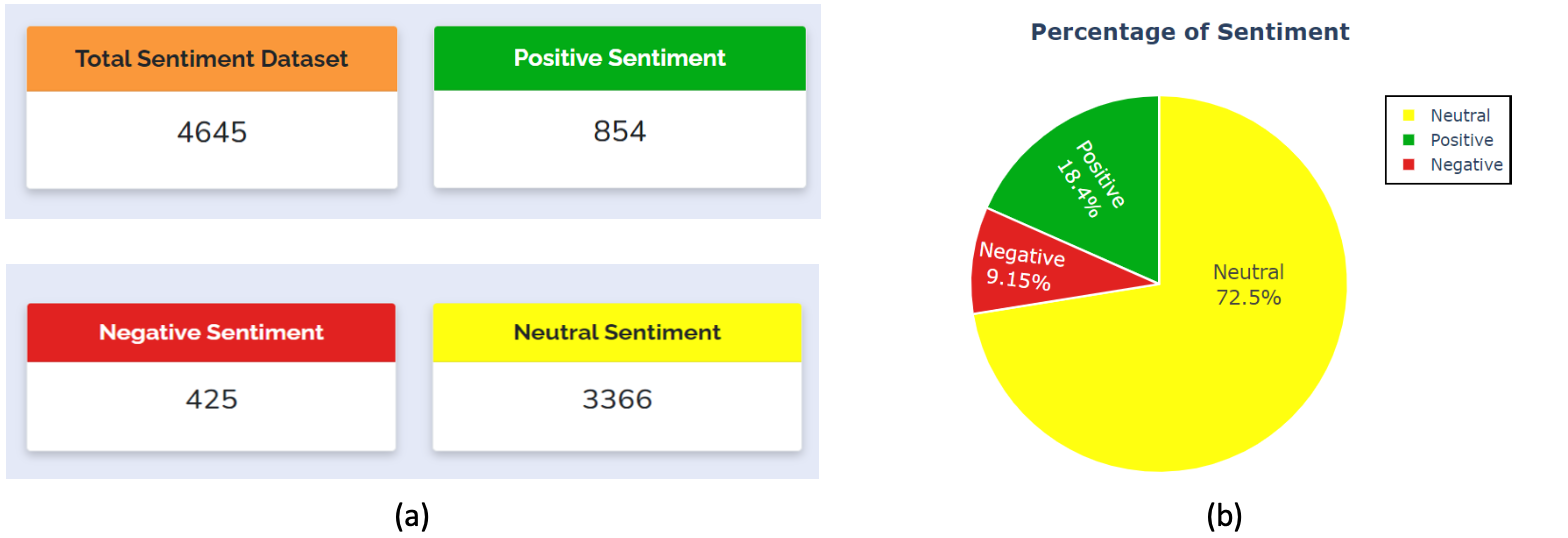
\includegraphics[width=0.8\textwidth]{BetterVisualizationsOfData.png}
    \caption{Example of visualization of data from study\cite{b2}}
\end{figure*}





\section{Proposed Methodology}

Our methodology attempts to explore self-supervised models further and at the same time, compare performance against supervised learning models. Based on our analysis of various academic papers we found that SVM was one of the most accurate models and decided to compare this to the BERTweet model for emotional recognition. 

\subsection{Data Collection}

We begin with the data collection step. 
We utilized 2 datasets from online sources. Both of these datasets were labelled so that we could evaluate the accuracy and performance of these models.
We are currently working with the Twitter US Airline Sentiment Dataset and the Weather dataset both which are very different in terms of the content. 
Our goal is to see how well our model could perform with datasets of different sizes and topics. 

\subsection{Data Preprocessing}
The next step is to process the data. 
In the preprocessing step, we assign target values to each tweet. This value would be assign "0" if the tweet is negative, "1" if it is neutral, and "2" if it is positive.  Where necessary, we also remove stopwords from our dataset and remove any links which are not necessary for our model. We also tokenize our text, which splits the text into smaller components. This is important so that our model can focus solely on the textual information presented. We then generate embeddings for each tweet in order to get a numerical representation to feed into our models. In our next step, we split the using 80\%  for training and 20\% for validation.


\subsection{Training/Finetuning}
Our next step is to finetune or train our models. We decided to test 3 different models in our analysis.

Our first model used the BERTweet model to classify tweet sentiment. BERT stands for Bidirectional Encoder Representations from Transformers. It is a deep learning model which was introduced by Google in 2018. This model makes use of a transformer which contains an attention mechanism. This allows the model to understand contextual relations between words in a text\cite{b17}.The BERTweet model is based off of this BERT but is pretrained on a large corpus of tweets, making it suitable for our task  \cite{b18}
We believe this is the appropriate model to use because we intend to test the ability of unsupervised models in this particular case and BERTweet is an effective model for this task.

 



Our second model used SVM to classify tweets. This model has been widely used and proven to achieve very accurate results. Prior to training this model we used Bag of Words model to generate embeddings to feed into the SVM classifier. The Bag of Words model is a way of representing text numerically by using a vacbulary of known words and measuring presence of known words to create a vector for a piece of text\cite{b19}.

Our third model used SVM to classify tweets however, we used BERTweet's model to generate embeddings prior to training this model. This is because we wanted to test whether it would be beneficial for us to use capabilities of both transformer models and supervised learning models to achieve good results. The BERT model is known for generating contextual embeddings which could potentially improve model accuracy\cite{b17}. 


\subsection{Classification}
Using our finetuned/trained model, we then evaluate our tweets based on positive, negative or neutral sentiment to allow us to determine sentiment on a particular issue. This classification is performed on the validation set.
We then aggregate all the predictions to get an overall view of the public sentiment given a particular dataset. 

\subsection{Visualization}
The next step is to visualize our data. 
Firstly, we use a word cloud which specifies all the key words indicating positive, negative, and neutral sentiment. 
An example of this can be shown below.

\begin{figure}[t]
    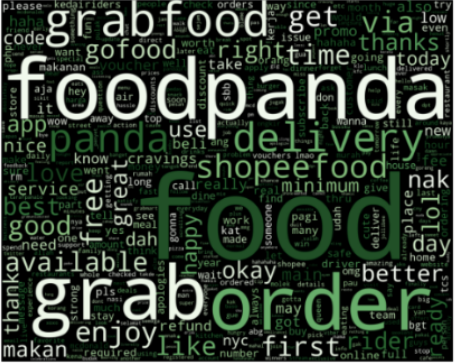
\includegraphics[width=0.5\textwidth]{wordcloud.png}
    \caption{Example of word cloud\cite{b2}}
\end{figure}

 We also included a pie chart showing the distribution of positive, negative and neutral tweets. 
 We will also add additional visualizations which we plan to show in the next step which is evaluating performance.
 In order to display this information to the user we will be implementing a web application using the Django Framework in python. 
 "Django is a high-level Python web framework that encourages rapid development \cite{b14}."
 Given our shorter time frame, we believe that this framework will be able to give us the best product within the fastest time frame.
 This is due to the fact that Django is consistent in their design principles and have lots of up-to-date documentation \cite{b15}. 


\subsection{Evaluation of Performance}
Evaluating the performance of our model involves a few metrics which need to be calculated. 
Prior to performing our calculations, we will display a confusion matrix which shows, true positives, true negatives, false positives, and false negatives in a matrix. 
An example in python is shown below:


\begin{figure}[b]
    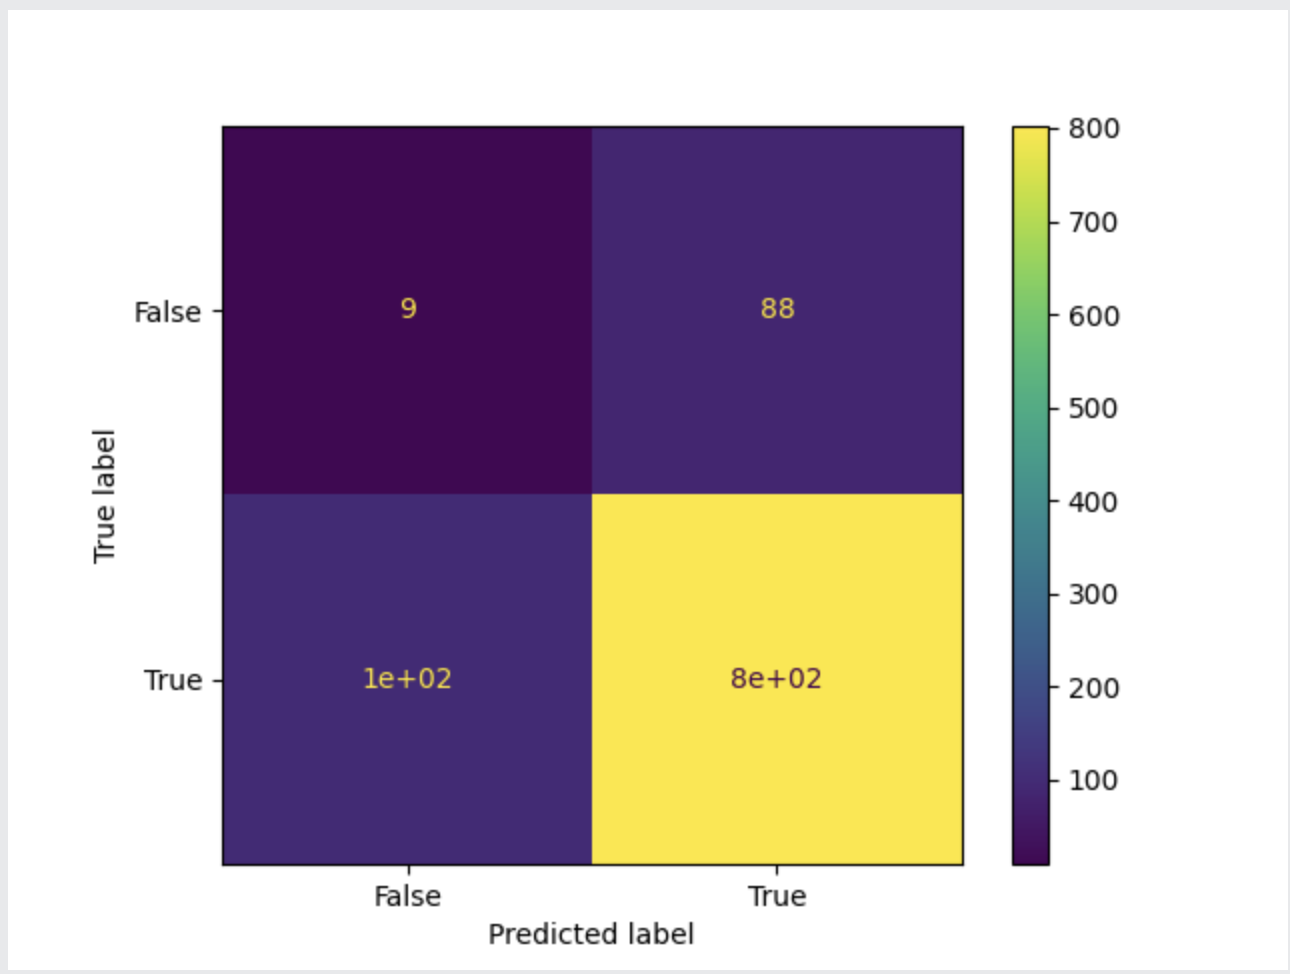
\includegraphics[width=0.5 \textwidth]{confusion_matrix.png}
    \caption{Example of confusion matrix in python\cite{b16}}    
\end{figure}
The confusion matrix will be used to calculate multiple metrics including accuracy, performance, recall, and F1 score, the equations of which are as follows:

\begin{align}
    Accuracy &= (TP + TN) / (TP + TN + FP + FN)\\
    F1 &= 2TP / (2TP + FP + FN)\\
    Precision &= TP / (TP + FP)\\
    Recall &= TP / (TP + FN)
\end{align}

\section{Datasets Description}
This section provides a detailed overview of two key datasets used in our analysis: the Swiggy Tweet dataset and the Twitter US Airline Sentiment dataset. 
Each dataset is unique in its focus and offers valuable insights into customer sentiment in different sectors.

\subsection{Weather Tweet Dataset}
\begin{itemize}
    \item \textbf{Description}: This dataset is a small set of data containing tweets that express sentiments on weather.
    
    \item \textbf{Weblinks}: \url{https://data.world/crowdflower/weather-sentiment}[10]
    
    \item \textbf{Type of Data}: It comprises mainly textual data from tweets, numerical data, and categorical data from user IDs and screen names.
    
    \item \textbf{Statistics}:
    \begin{itemize}
        \item \textit{Number of Instances}: The dataset comprises 1000 tweets, allowing us to test performance of our models smaller datasets.
        \item \textit{Number of Columns}: 10 columns provide varied data points including engagement metrics, user demographics, and textual content for in-depth analyses.
        \item \textit{Unique Tweets}: Out of 1000 tweets, 1000 are unique, indicating an almost negligible level of repetition and emphasizing the originality of the dataset.

    \end{itemize}
\end{itemize}

\subsection{Twitter US Airline Sentiment Dataset}
\begin{itemize}
    \item \textbf{Description}: The Twitter US Airline Sentiment dataset is composed of tweets aimed at US airlines, tagged with sentiments to enable a detailed sentiment analysis. With 14,640 instances, the dataset records sentiments as negative, neutral, or positive, alongside the reasons for negative sentiments, offering a comprehensive look into public opinion on airline services.
    
    \item \textbf{Weblinks}: \url{https://www.kaggle.com/datasets/crowdflower/twitter-airline-sentiment/data}[11]
    
    \item \textbf{Type of Data}: This dataset is primarily textual, with tweets labeled for sentiment analysis. It includes numerical data for sentiment confidence levels and retweet counts, and categorical data on airlines and reasons for negative feedback.
    
    \item \textbf{Statistics}:
    \begin{itemize}
        \item \textit{Number of Instances}: With 14,640 tweets, this dataset is a substantial corpus for analyzing public sentiment towards US airlines.
        \item \textit{Number of Columns}: The dataset is detailed across 15 columns, encompassing tweet IDs, sentiment analysis, reasons for negative sentiments, and user engagement statistics, thereby facilitating a comprehensive evaluation of airline services.
        \item \textit{Unique Tweets}: There are 14,427 unique tweets, ensuring the dataset's diversity and reducing bias from duplicate entries.
        \item \textit{Average Retweet Count}: An average retweet count of approximately 0.083 per tweet indicates the social sharing dynamic and reach of these customer experiences.
        \item \textit{Sentiment Distribution}: The breakdown of sentiments as 9,178 negative, 3,099 neutral, and 2,363 positive, underscores the prevalence of negative sentiment in the dataset.
    \end{itemize}
    The statistical insights provided above were derived using the pandas library,open-source software library written for data analysis in Python[12].

\end{itemize}


\section{Implementation Requirements}
In this section, we delve deeper into the technologies selected for our sentiment analysis project on Twitter data, elaborating on their roles and integration points within the application.

\begin{itemize}

    \item \textbf{Google Colab}: As our models require heavy computational power, we utilized Google Colab's runtime to execute our code. Google colab allows us to run Jupyter notebooks in a cloud hosted environment and allows us to perform heavy machine learning tasks.
    
    \item \textbf{Python}: As our primary programming language, Python's flexibility and comprehensive ecosystem are pivotal. It will serve multiple roles: data preprocessing, integration with machine learning models to refine or retrain BERTweet for enhanced accuracy, and driving our backend development with APIs for fetching analysis results, user management, and processed data delivery, leveraging the extensive capabilities of the Django framework. Python serves as the glue between the data and the sentiment analysis models. With libraries such as TensorFlow, we can further refine or even retrain models like BERTweet based on specific needs or to improve accuracy.
    
    \item \textbf{Django Framework}: The Django Framework is selected for its robustness, scalability, and ease of integration with Python's data science and machine learning libraries. It facilitates the rapid development of secure and maintainable web applications, providing out-of-the-box support for common web development tasks. This includes a powerful admin interface for easy data model management, making it simpler to handle large volumes of traffic and data efficiently. Django's security features protect our application from common vulnerabilities, ensuring a secure user experience. With Django, our backend is not only highly scalable but also adaptable, allowing our application to grow seamlessly as user demands and technologies evolve.
    
    \item \textbf{BERTweet}: BERTweet, a model trained specifically on tweets using BERT (Bidirectional Encoder Representations from Transformers), is central to our project for performing sentiment analysis. It excels at classifying tweets into various sentiments and uncovering trends in public opinion, thanks to its training on a vast array of Twitter messages. This specialized focus on tweets means BERTweet is adept at understanding the nuances of short, informal text commonly found on social media. This capability makes it exceptionally suited for real-time analysis, offering insights into the public's reactions and sentiments on different topics, thereby enriching our project's analytical depth.

    \item \textbf{Additional Tools and Libraries}: Our project leverages the power of Pandas and NumPy for efficient data manipulation and analysis. These libraries are fundamental for working with large datasets, allowing us to organize, clean, and analyze data with high performance and flexibility. For visualization, we turn to Matplotlib and Seaborn, which enable us to create informative and attractive visualizations. These tools help us to present our findings in a clear and accessible way, through charts, graphs, and dashboards that highlight key trends and insights derived from our sentiment analysis. This visual component is vital for communicating complex data in an understandable format to users. For our machine learning workloads, we utilized libraries such as nltk, sklearn, torch and transformers which were useful in various tasks including tokenization, embedding, model training, evaluation and visualization.
\end{itemize}
The combination of these technologies and frameworks enabled  the development of a comprehensive web application that leverages advanced sentiment analysis to provide valuable insights into various datasets, thereby meeting our project objectives.

\section{Results}
Our results proved to be quite meaningful and relevant. Our analysis focuses mostly on the Airline U.S Sentiment dataset as that contained a robust amount of tweets for analysis. The weather dataset was for testing model performance on smaller datasets. Below is a pie chart showing the distribution of positive, negative and neutral tweets. In addition to word clouds of positive, negative, and neutral words present in our data.

/* insert images here (word clouds and pie chart for Airline Dataset) */

As you can see, our data consists of predominantly negative tweets. After running our model on the validation set, the following are the results we achieved for each model.

/*include confusion matrices here for all models*/
/*included accuracy precision and recall for models as well*/

Looking at the data it is evident that the SVM model using BOW performed significantly worse than the other 2 models. This is expected because this dataset of over 14000 tweets is not enough to train the SVM model with good results. 

The best performing model overall was the BERTweet model which was also expected because this model was pretrained on millions of tweets and is expected to perform better for this dataset. One thing which was unexpected was that the SVM model that used BERTTweet embeddings had results which compared well to the BERTweet model. This was very impressive and unexpected. Using BERTweet for embeddings proved that we can achieve better results due to the fact that BERTweet provides contextual embeddings which are more accurate representations of tweets, to the SVM model. The accuracy of this model was only 1\% worse for this dataset. In addition, its precision on the neutral class was better than the BERTweet model indicating that it performs more accurate predictions on neutral tweets than the BERTweet classification model. Its recall on the negative class performed better as well showing that out of all the negative tweets, this SVM model classified more of these negative than the first BERTweet model.
Although the BERTweet model metrics were better overall, the SVM model is still competitive due to the fact that it is much less computationally expensive.  The BERTweet model took almost 17 minutes to train while the SVM model using BERTweet embeddings used only 5 minutes to generate embeddings and 32 seconds to train. Overall our objective was accomplished in that we were able to produce better visualizations and come up with a methodology that was more suitable for situations where computational resources are limited. In addition to this test, we also applied this methodology to a smaller dataset, to see what would happen in cases where data is limited. We used a dataset of 1000 tweets on weather data to test this. The following were the results:

/*included accuracy precision and recall for all models on we*/

According to these results, we realized that BERTweet significantly outperforms the other two models however, there are a few metrics in which BERTweet embeddings + SVM does slightly better. The recall for the negative class and precision for positive class for BERTweet embeddings + SVM is better however, these metrics dont matter considering the fact that it is outperformed by the BERTweet model in almost every category. Our suggestion is to use BERTweet on data that is limited as this model has already been pretrained on a large corpus of tweets and doesnt require as much finetuning. 


\begin{thebibliography}{00}
\bibitem{b1} F. Benrouba and R. Boudour, "Emotional sentiment analysis of social media content for Mental Health Safety," Social Network Analysis and Mining, vol. 13, no. 1, 2023. \url{doi:10.1007/s13278-022-01000-9}
\bibitem{b2} A. F. A. Samah et al., "Aspect-Based Classification and Visualization of Twitter Sentiment Analysis Towards Online Food Delivery Services in Malaysia," View of aspect-based classification and visualization of Twitter sentiment analysis towards online food delivery services in Malaysia, 2024. [Online]. Available: \url{https://doi.org/10.37934/araset.37.1.139150} [Accessed: Mar. 23, 2024]
\bibitem{b3} Bhavnani, H.D. (2022) Developing an emotion recognition tool for tweets, Cloud Computing and Data Science. Available at: \url{https://doi.org/10.37256/ccds.4120231827} (Accessed: 23 March 2024). 
\bibitem{b4} Kavitha, D.N., Prasad Reddy, P.V. and Venkata Rao, K. (2023) ‘Emotion recognition in tweets using optimized SVM and Knn Classifiers’, Lecture Notes in Electrical Engineering, pp. 135–144. \url{doi:10.1007/978-981-19-8865-3_12}
\bibitem{b5}Susmitha, C. et al. (2023) Sentimental Analysis on Twitter Data using Supervised Algorithms, Request rejected. Available at: \url{doi:10.1109/ICCMC56507.2023.10084278} (Accessed: 23 March 2024).
\bibitem{b6} Kanade, V. (2022) All you need to know about support vector machines, Spiceworks. Available at: \url{https://www.spiceworks.com/tech/big-data/articles/what-is-support-vector-machine/#:~:text=A%20support%20vector%20machine%20(SVM)%20is%20a%20machine%20learning%20algorithm,classes%2C%20labels%2C%20or%20outputs.}
\bibitem{b7} ProjectPro (2023) Bert NLP model explained for complete beginners, ProjectPro. Available at: \url{https://www.projectpro.io/article/bert-nlp-model-explained/558} (Accessed: 23 March 2024)
\bibitem{b8} ALBU, I.-A. and SPÎNU, S. (2022) EMOTION DETECTION FROM TWEETS USING A BERT AND SVM ENSEMBLE MODEL, VAPOR LIQUID. Available at: \url{https://arxiv.org/ftp/arxiv/papers/2208/2208.04547.pdf} (Accessed: 2024). 
\bibitem{b9} Shah, D. and Jha, A. (2023) Self-supervised learning and its applications, neptune.ai. Available at: \url{https://neptune.ai/blog/self-supervised-learning#:~:text=Self%2Dsupervised%20learning%20is%20a,as%20predictive%20or%20pretext%20learning.}(Accessed: 23 March 2024). 
\bibitem{b10} Shrijayan (2022) Sentimental analysis, Kaggle. Available at: \url{ https://www.kaggle.com/datasets/cpluzshrijayan/swiggy-tweet} (Accessed: 23 March 2024).  
\bibitem{b11} Eight, F. (2019) Twitter us airline sentiment, Kaggle. Available at: \url{https://www.kaggle.com/datasets/crowdflower/twitter-airline-sentiment} (Accessed: 23 March 2024). 
\bibitem{b12} Lewis, H. (2020) Getting started with pandas in Python, Getting Started with pandas in Python | UVA Library. Available at: \url{https://library.virginia.edu/data/articles/getting-started-with-pandas-in-python} (Accessed: 23 March 2024). 
\bibitem{b13} Quoc Nguyen , D.Q.N.,  Vu, T. and Tuan Nguyen., A. (2020) BERTweet, BERTweet. Available at: \url{https://huggingface.co/docs/transformers/en/model_doc/BERTweet} (Accessed: 24 March 2024). 
\bibitem{b14} Django Software Foundation, (2024) Django: The Web framework for perfectionists with deadlines, Available at: \url{https://www.djangoproject.com} (Accessed: 25 March 2024)
\bibitem{b15} Mozilla Contributors, (2024) Introduction to Django, Available at: \url{https://developer.mozilla.org/en-US/docs/Learn/Server-side/Django/Introduction} (Accessed: 25 March 2024)
\bibitem{b16} W3Schools, Machine Learning - Confustion Matrix, Available at: \url{https://www.w3schools.com/python/python_ml_confusion_matrix.asp} (Accessed: 23 March 2024)
\bibitem{b17} Horev, R. (2018) BERT Explained: State of the art language model for NLP, Available at: \url{https://towardsdatascience.com/bert-explained-state-of-the-art-language-model-for-nlp-f8b21a9b6270} (Accessed: 23 March 2024)
\bibitem{b18} Hugging Face, BERTweet Documentation, Available at: \url{https://huggingface.co/docs/transformers/en/model_doc/BERTweet} (Accessed: 23 March 2024)

\bibitem{b19} A gentle introduction to the Bag of Words Model, Available at: \url{https://machinelearningmastery.com/gentle-introduction-bag-words-model/} (Accessed: 23 March 2024)
\end{thebibliography}
\vspace{12pt}
\end{document}
